%   Filename    : chapter_4.tex 
\chapter{System Prototype}
%This chapter  presents the preliminary results or the system prototype of your SP.

\section{User Interface}
The mid-fidelity wireframe of the application’s features will be subdivided into three interfaces, namely PNP Admin, User or Main, and Companion.

\subsection{PNP Admin Interface}
The PNP-side interface will focus on the managing and administrative side of the product. Figure \ref{fig:PNP1} Login page of the PNP-side app will authenticate the user to enforce access in the reports management system of the missing persons. Input fields are provided for username and password for PNP’s credentials. When the PNP Admin user is having troubles with regards to authentication or registration, he/she would need to contact the developers directly, either to get an admin account for their respective PNP outpost, or to reset the password of their said admin accounts.
\begin{figure}[!h]
    \centering
    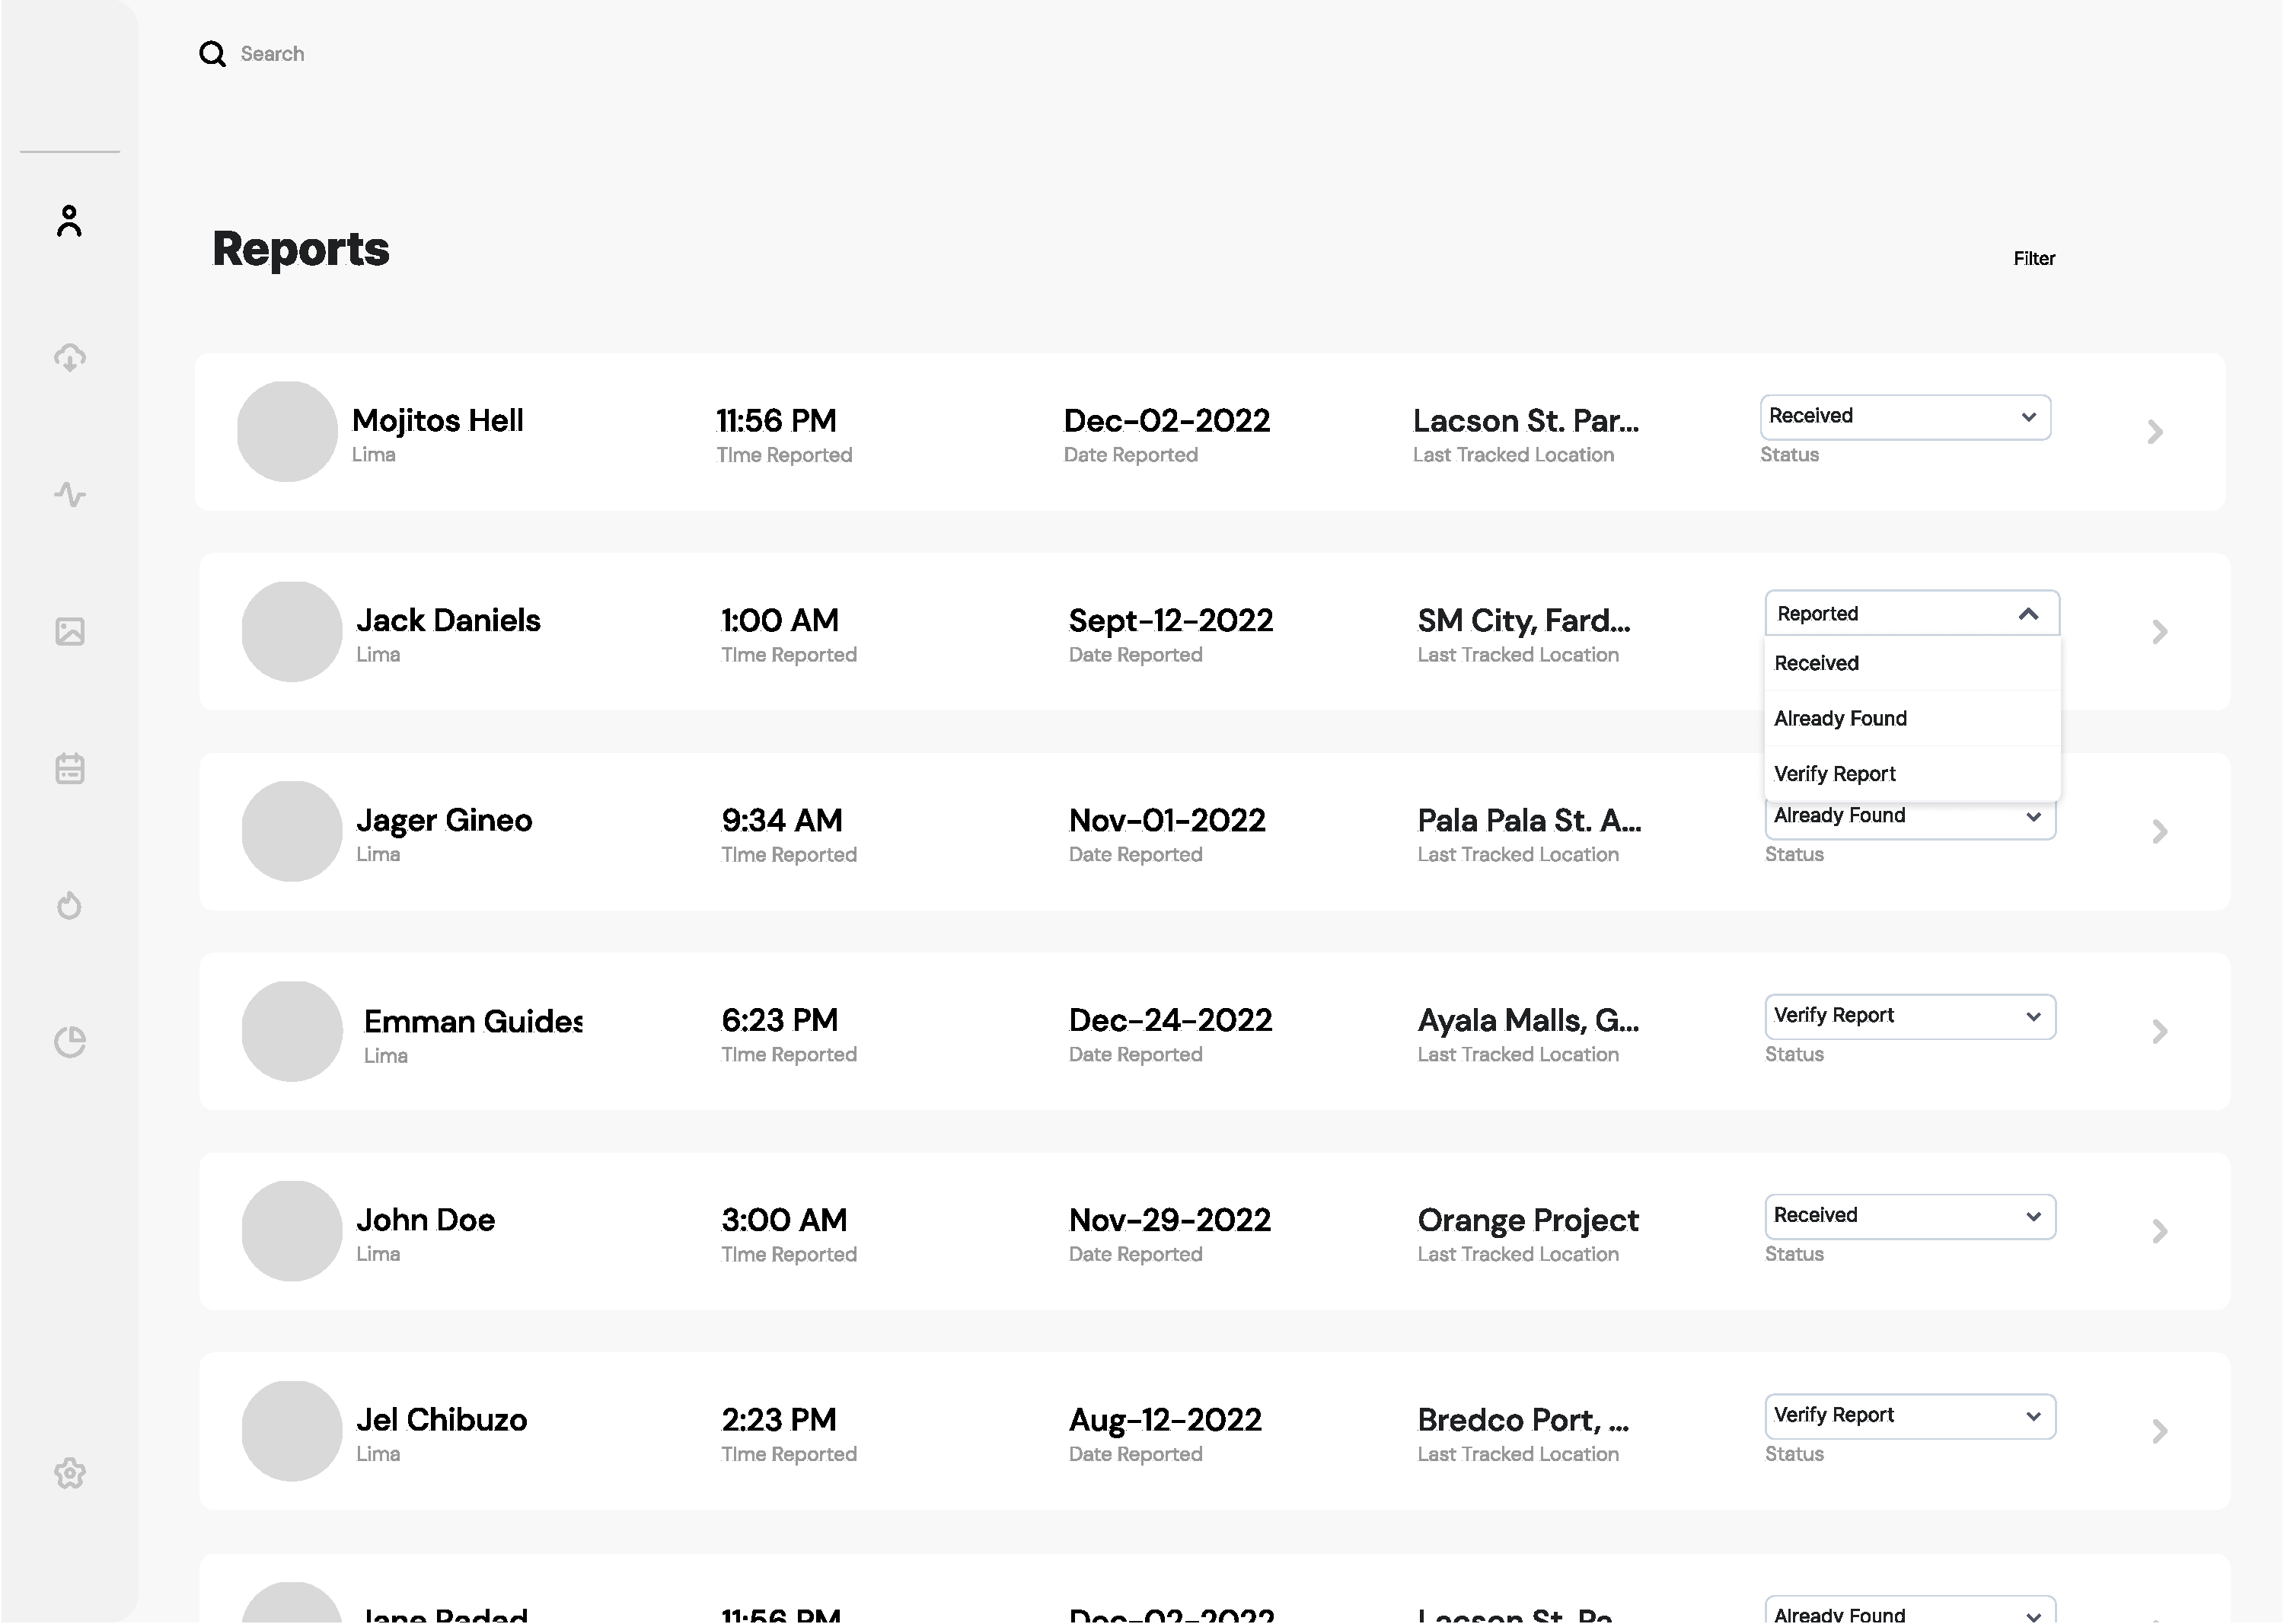
\includegraphics[scale=0.25]{interface/PNP/PNPDesktop1.pdf}
    \caption{Desktop View for Login Page}
    \label{fig:PNP1}
\end{figure}

\begin{figure}[!h]
    \centering
    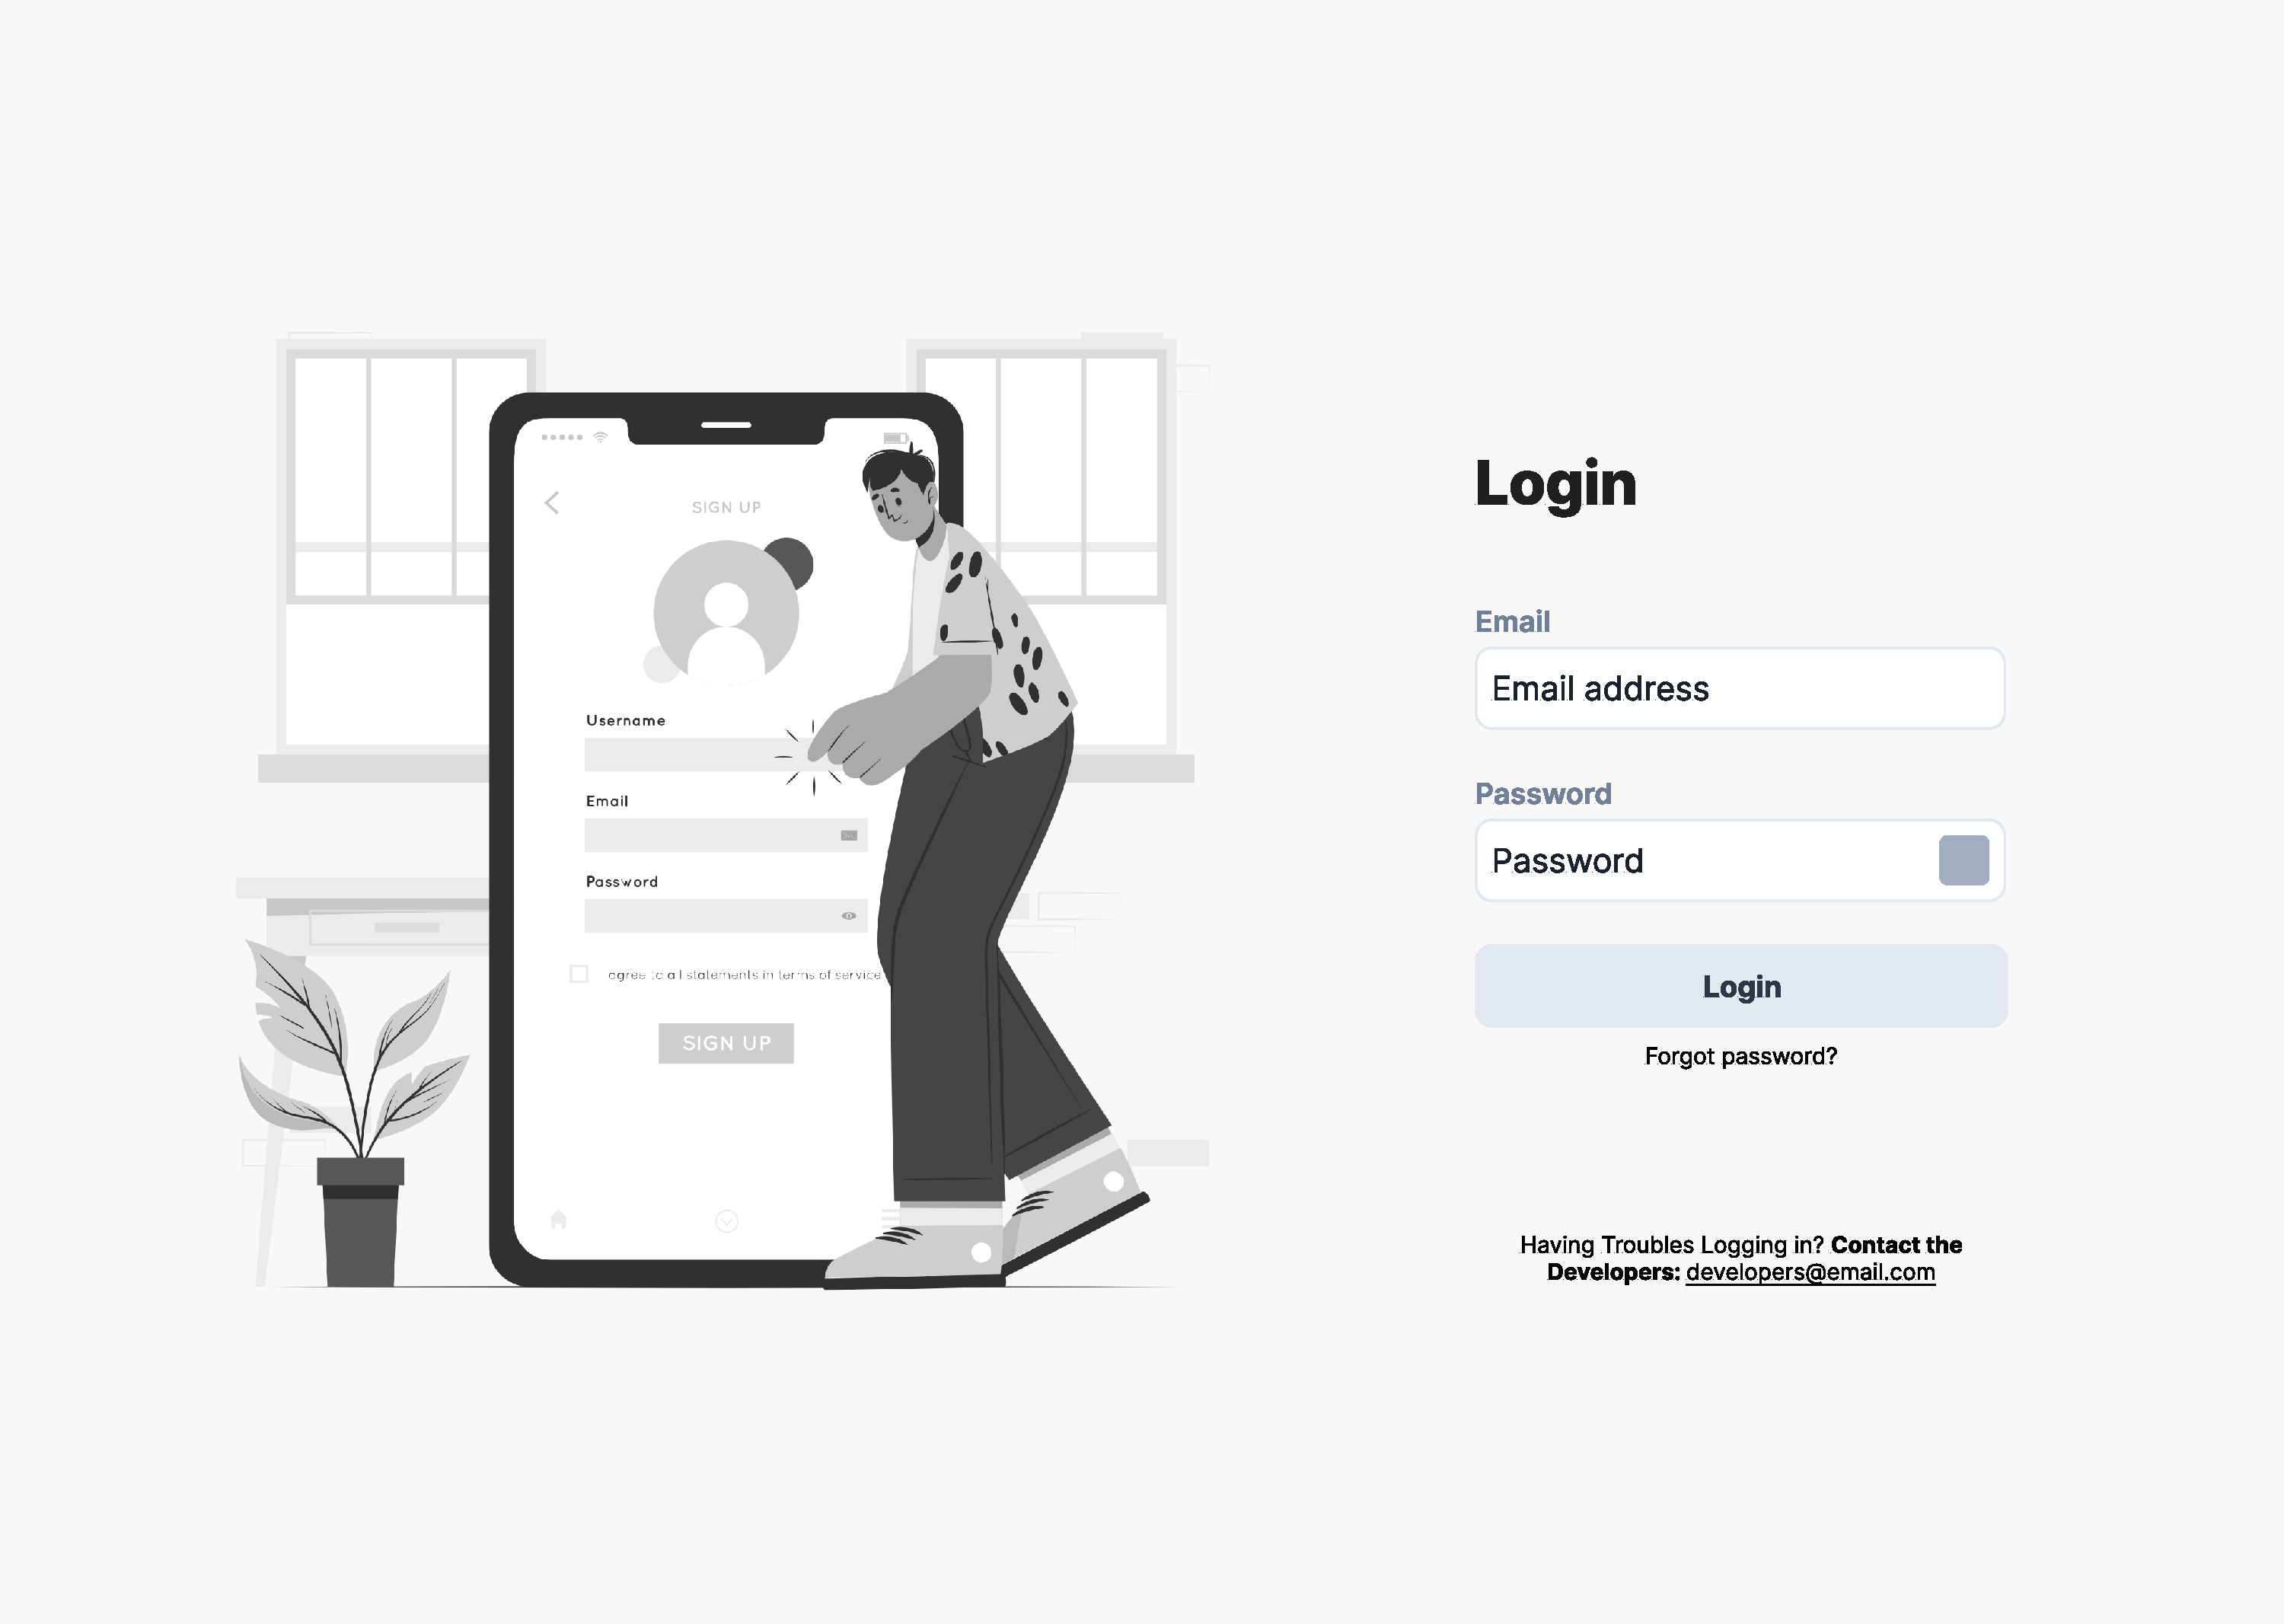
\includegraphics[scale=0.25]{interface/PNP/PNPDesktop2.pdf}
    \caption{Desktop View for Reports}
    \label{fig:PNP2}
\end{figure}
Figure \ref{fig:PNP2} is the management suite for the PNP to access reports. The Reports page will have a scrollable list that will consist of the various details such as MP’s name, status of the report, time and date reported, and the location of MP. As for the status, a dropdown menu will be used to categorize each report namely, Received, Already Found, Verify Report, and Reported. For better management, a Filter button located at the top-right will be available to ensure that every report is being noticed and filtered out.

\subsection{User or Main Interface}
\begin{figure}[!h]
    \centering
    \begin{minipage}[c]{0.50\linewidth}
        \centering
        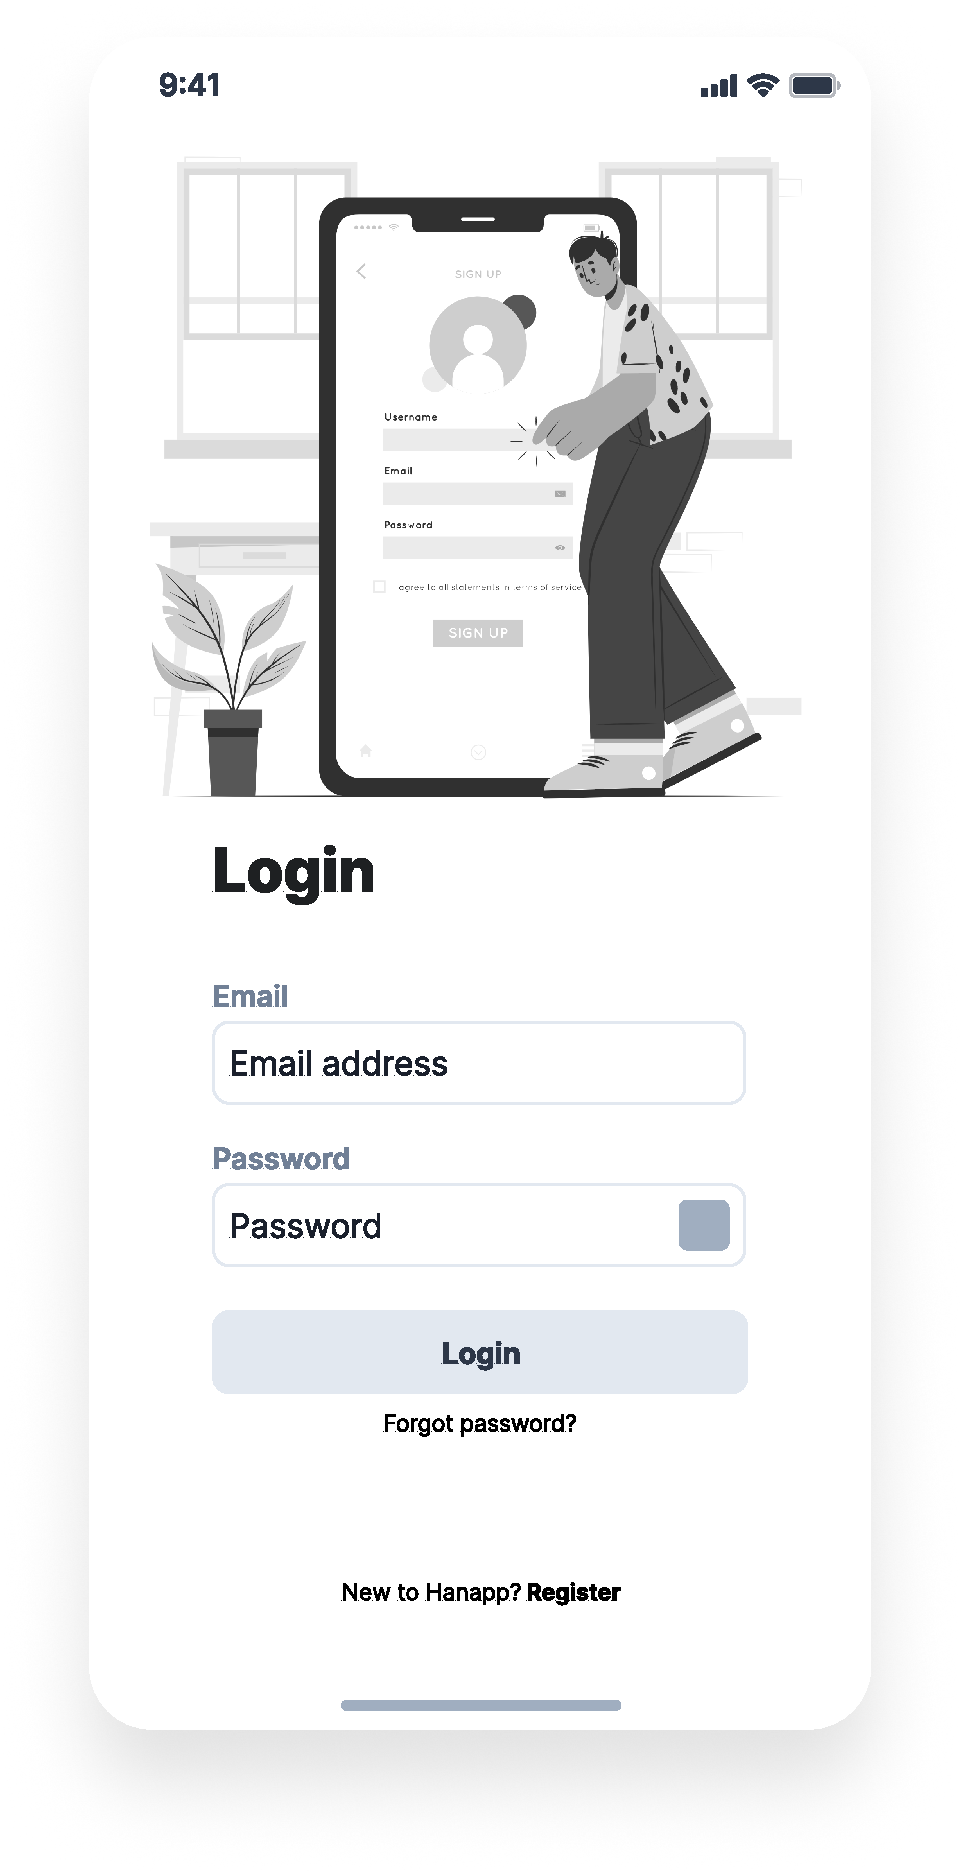
\includegraphics[scale=0.30]{interface/user/Login.pdf}
        \caption{Login Page}
        \label{fig:userLogin}
    \end{minipage}\hfill
    \centering
    \begin{minipage}[c]{0.50\linewidth}
        \centering
        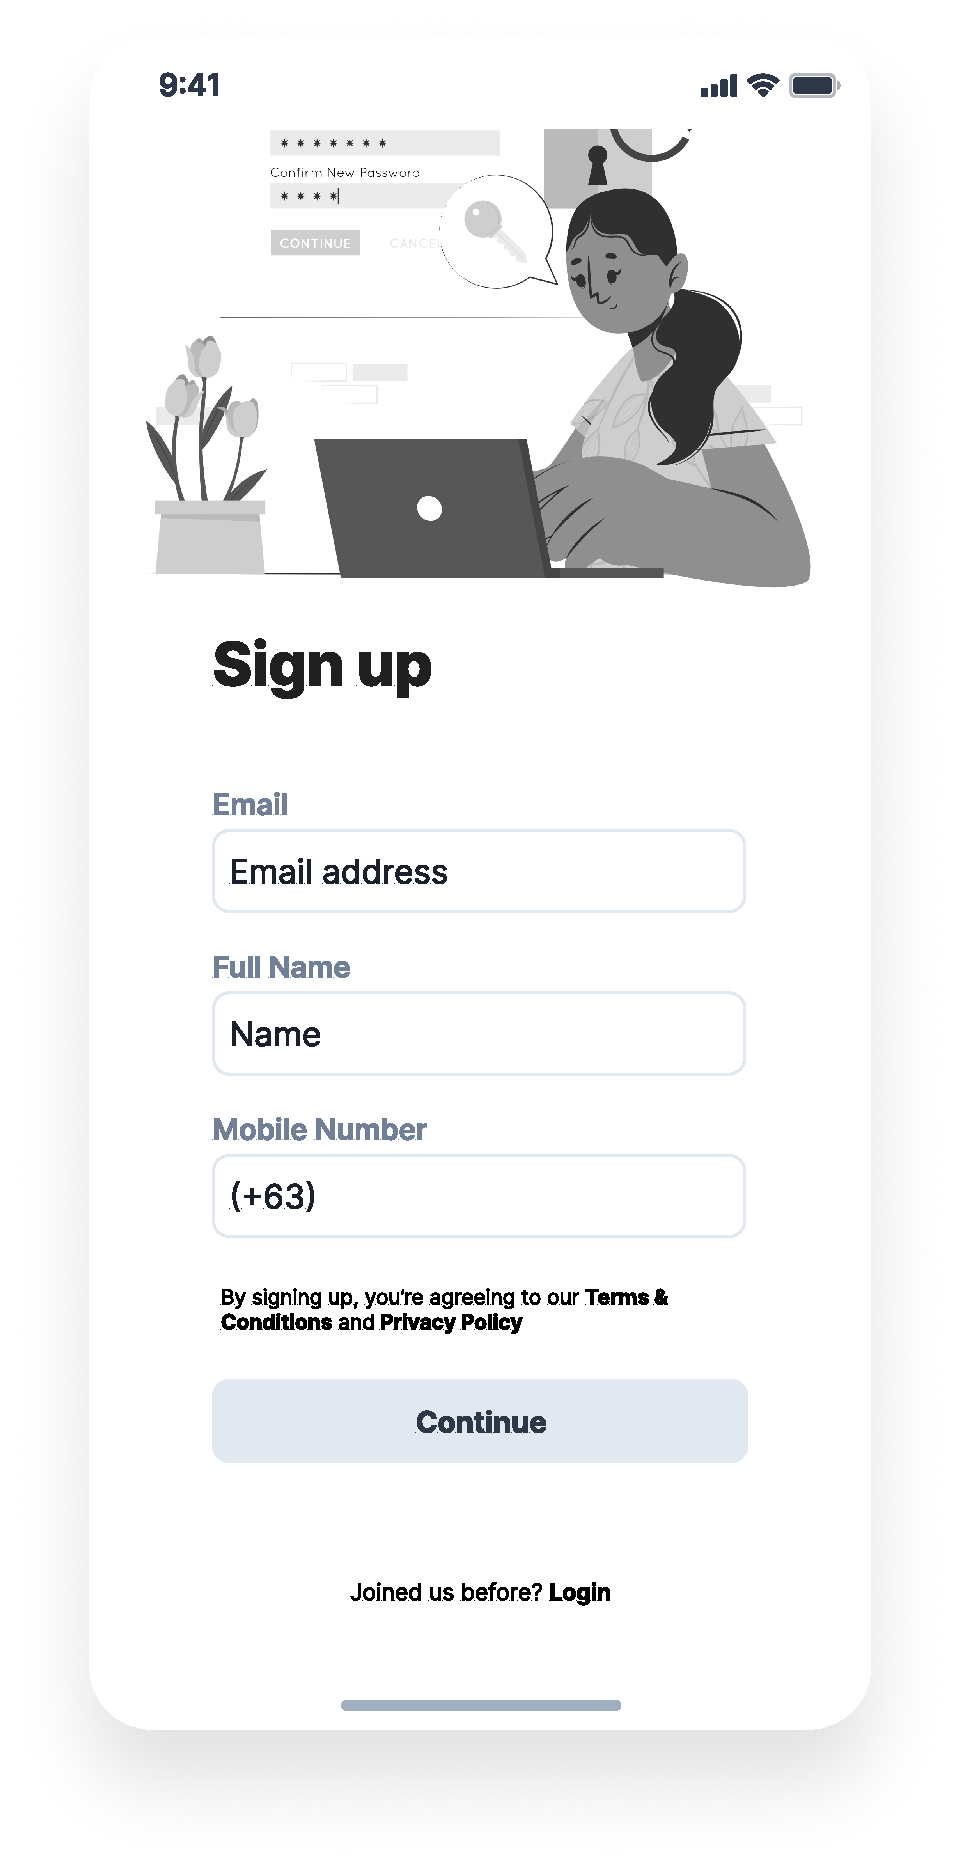
\includegraphics[scale=0.30]{interface/user/Register.pdf}
        \caption{Register Page}
        \label{fig:userRegister}
    \end{minipage}
\end{figure}
Authentication is necessary for the user-side. Figures \ref{fig:userLogin} and \ref{fig:userRegister} are the Login and Register page, respectively. Input fields will be provided for the registration, username and full name, a numeric input field will be observed for the mobile number. To ensure that the user understands the Terms and Conditions and Privacy Policy, a hyperlinked text can be used to redirect them for their perusal. Then a continue button will let the user proceed to the next required details such as reportee’s identification for easy reporting of missing persons later on.

\begin{figure}[!h]
    \centering
    \begin{minipage}[c]{0.50\linewidth}
        \centering
        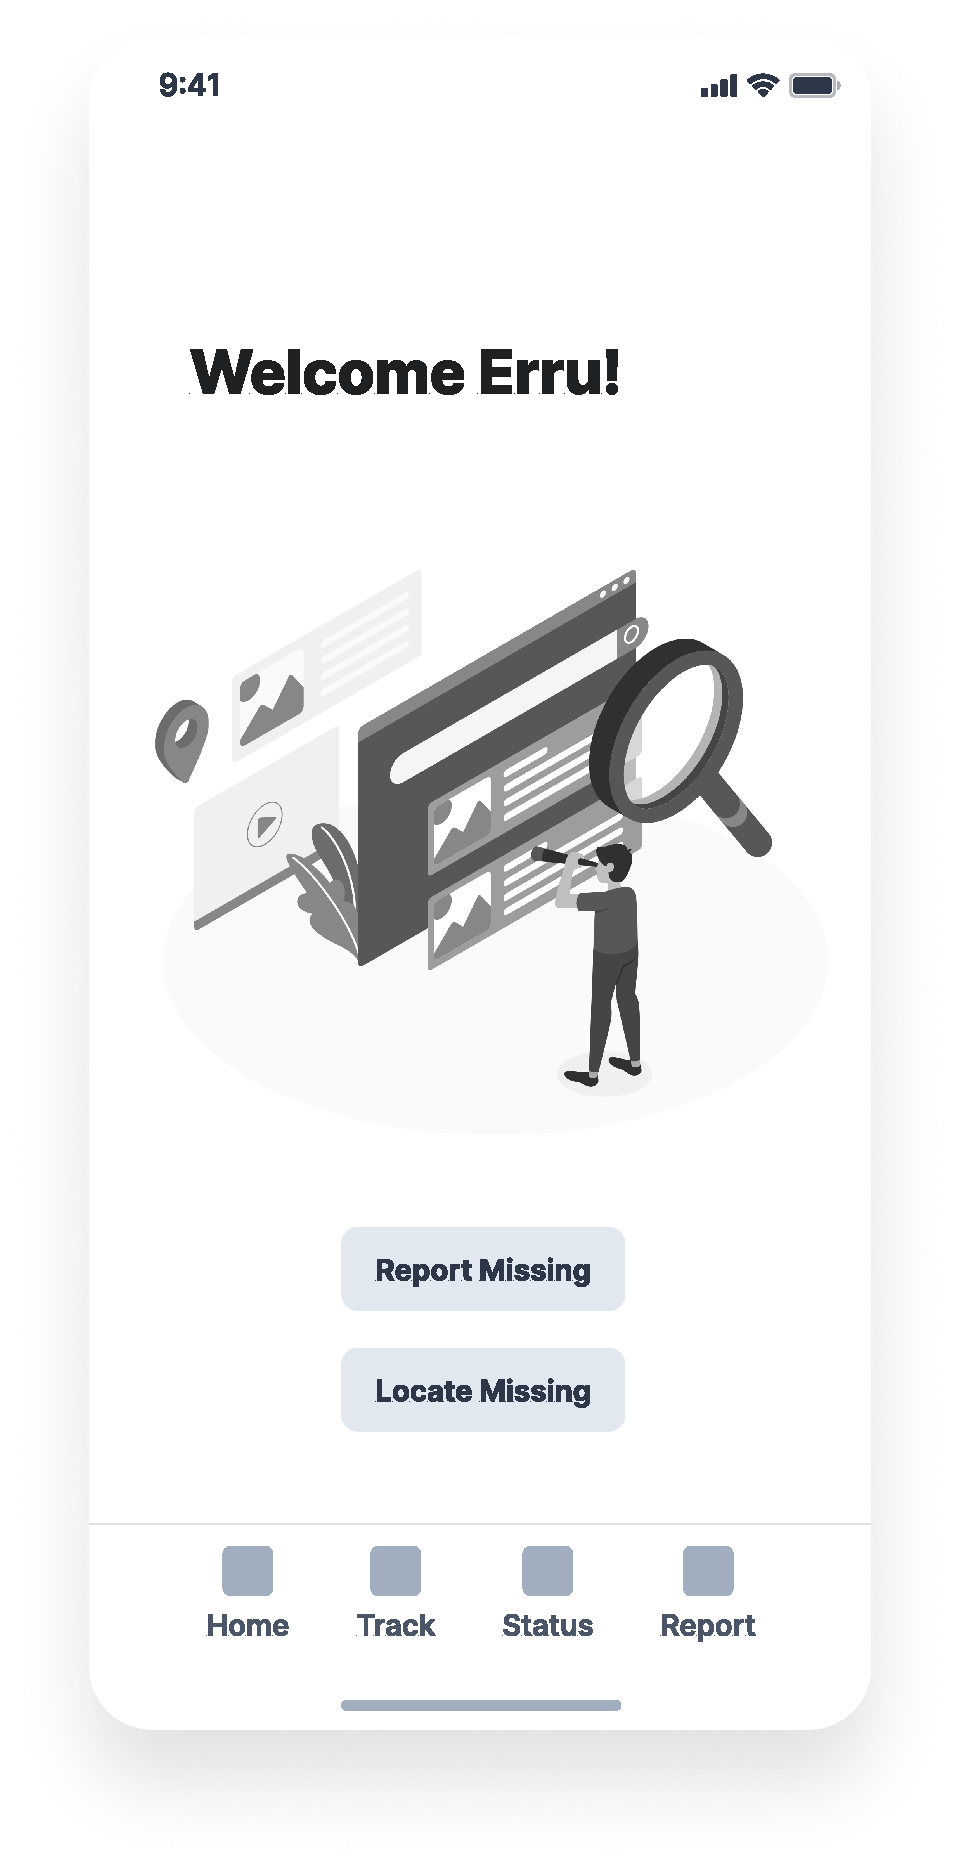
\includegraphics[scale=0.30]{interface/user/Home.pdf}
        \caption{Home Page}
        \label{fig:userHome}
    \end{minipage}\hfill
    \centering
    \begin{minipage}[c]{0.50\linewidth}
        \centering
        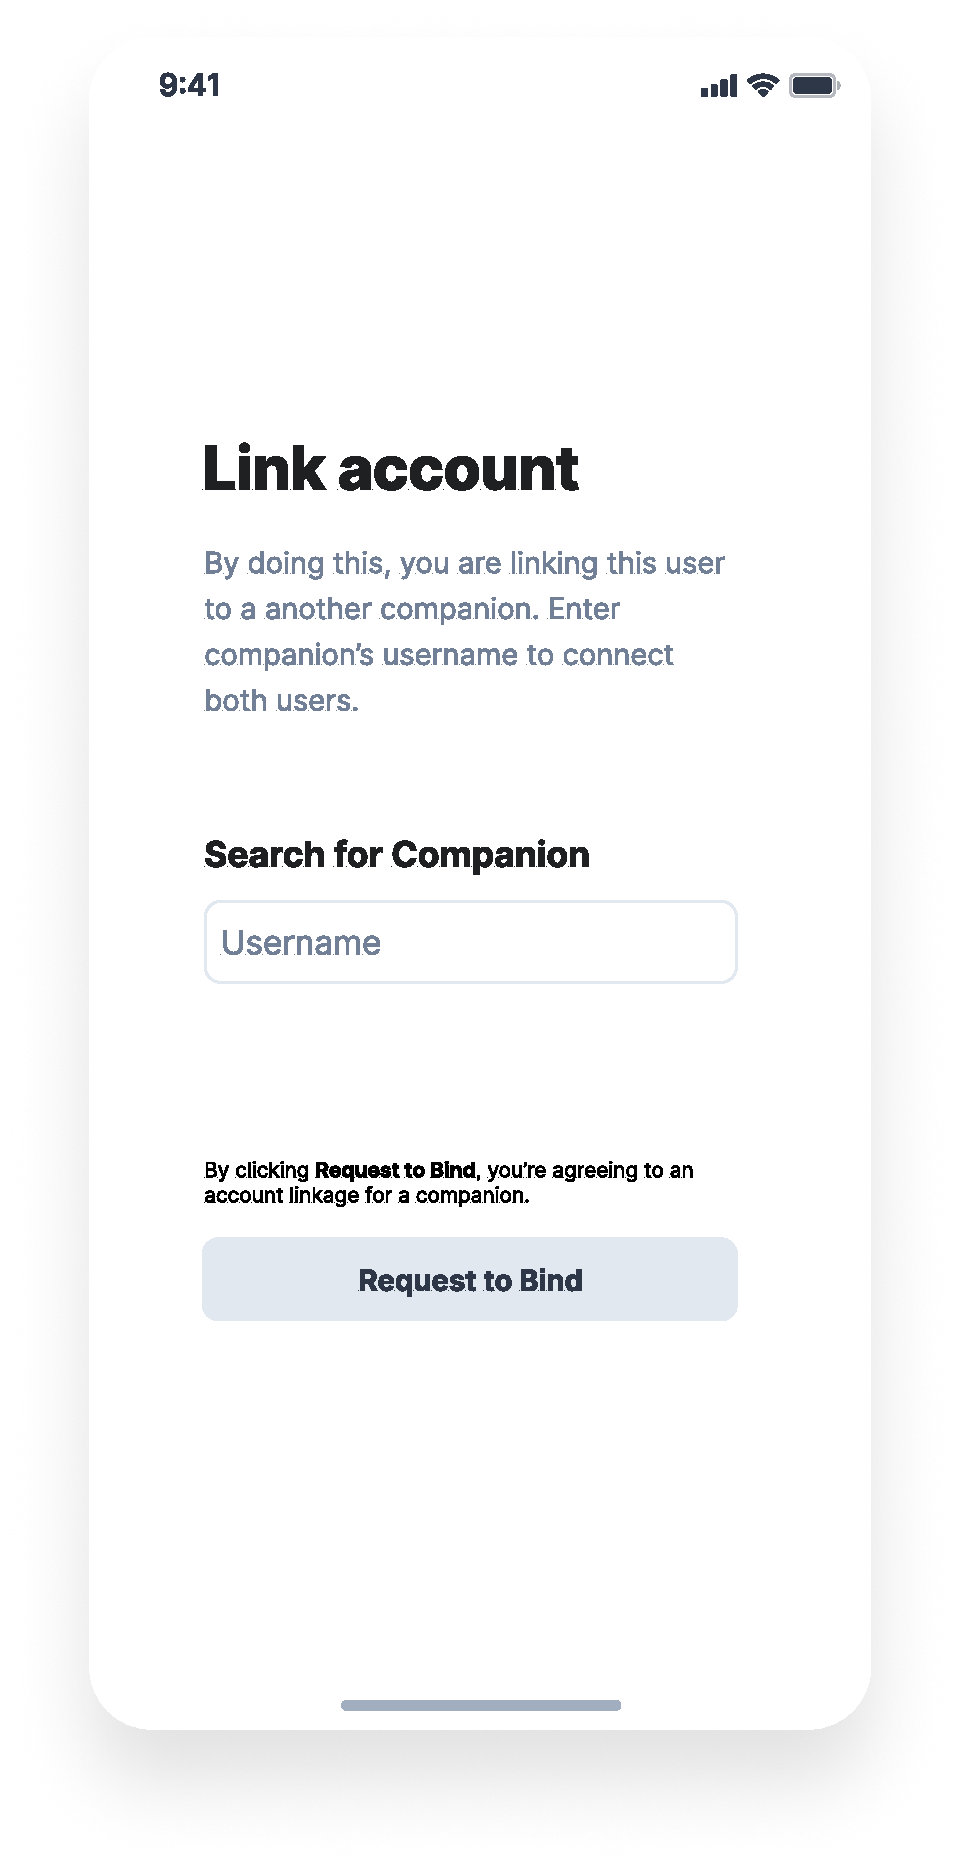
\includegraphics[scale=0.30]{interface/user/LinkAccount.pdf}
        \caption{Link Account Section}
        \label{fig:userLink}
    \end{minipage}
\end{figure}
Moreover, when user authentication is completed. The login button will let them proceed to the Home page of the application where the user will have two options: Report Missing or Locate Missing persons. A bottom navigation bar will be visible throughout the user’s interaction of the app assuring that they can easily navigate the entire features offered to them. The navigation bar will consist of four (4) sections namely, Home, Track, Status, and lastly, Report. Each of these sections have distinct functionalities.
\\\\Importantly, the user-side application will be able to link user’s app to a companion app. Figure \ref{fig:userLink} searches unique companion’s username to bind both account for easy linkage of current location and for tracking purposes.

\begin{figure}[!h]
    \centering
    \begin{minipage}[c]{0.50\linewidth}
        \centering
        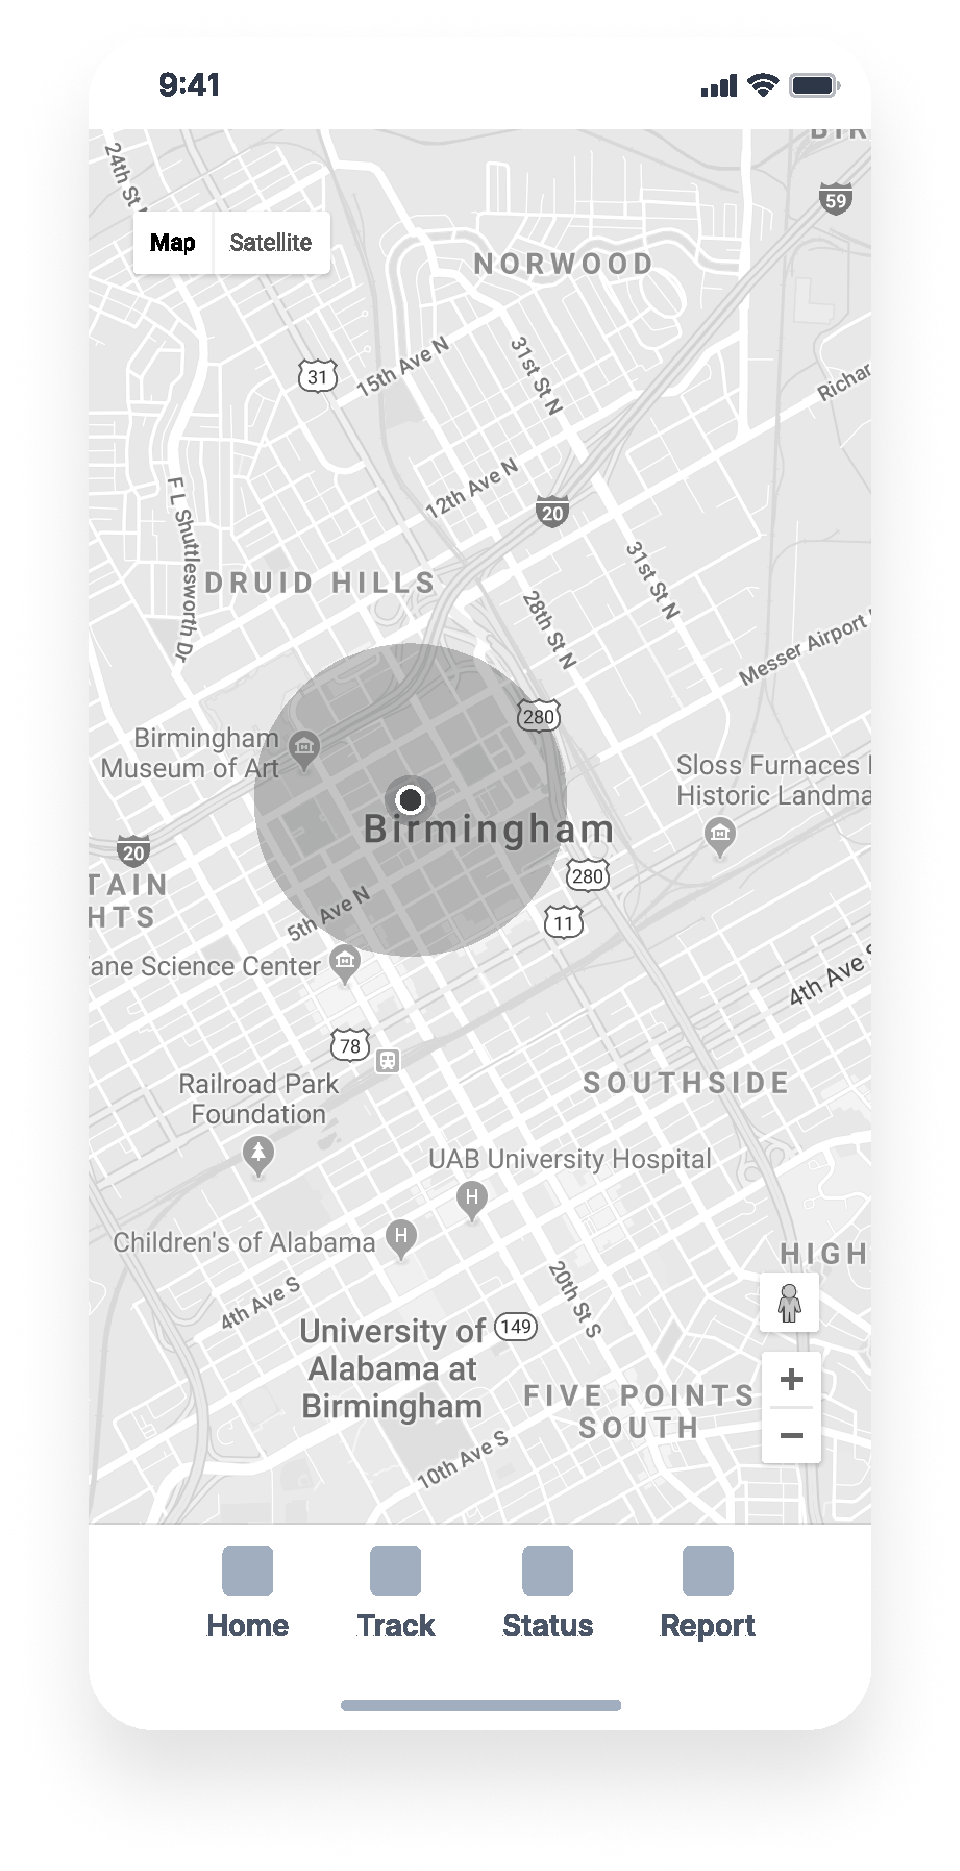
\includegraphics[scale=0.30]{interface/user/Tracking.pdf}
        \caption{Tracking MP Location}
        \label{fig:userTracking}
    \end{minipage}\hfill
    \centering
    \begin{minipage}[c]{0.50\linewidth}
        \centering
        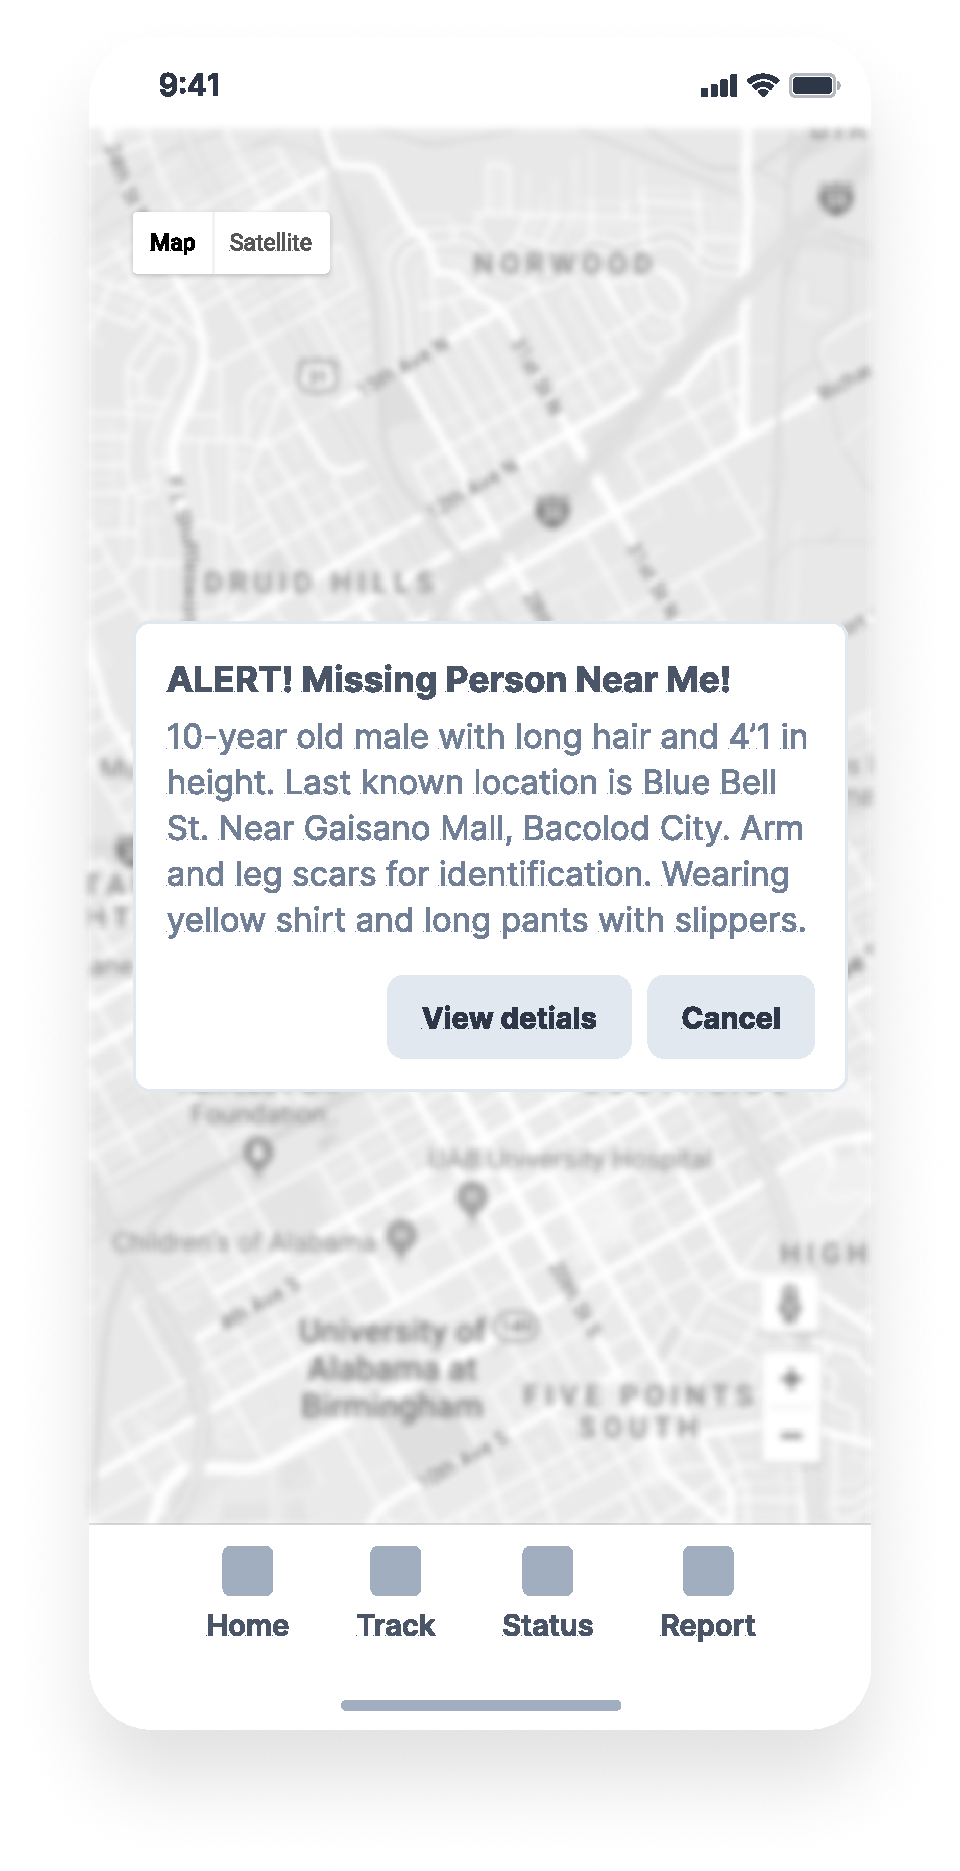
\includegraphics[scale=0.30]{interface/user/Notif.pdf}
        \caption{Push Notification Alert}
        \label{fig:userNotif}
    \end{minipage}
\end{figure}
Figure \ref{fig:userTracking} is the interface of tracking missing persons near the user. A location marker will guide the current or last seen whereabouts of a missing person. Apart from that, the user has the liberty to navigate the map, may it be street view or city-wide view by clicking the “person” icon at the lower right of the screen. Also, users can zoom in and zoom out depending on their preference. Considering, for example, that a 5-km radius will be visible, it will then encircle the last place the MP was seen.

As for the push notifications of incoming verified missing persons, Figure \ref{fig:userNotif} will prompt an alert message that will shortly disrupt the app’s activity. This way, the user’s attention is engaged and focused on the notification for a short period of time. The message will be a short description of the person in case there are sightings of them around the area. To give the user some leeway, they will have two options whether to view the details of the report or cancel the alert.

\begin{figure}[!h]
    \centering
    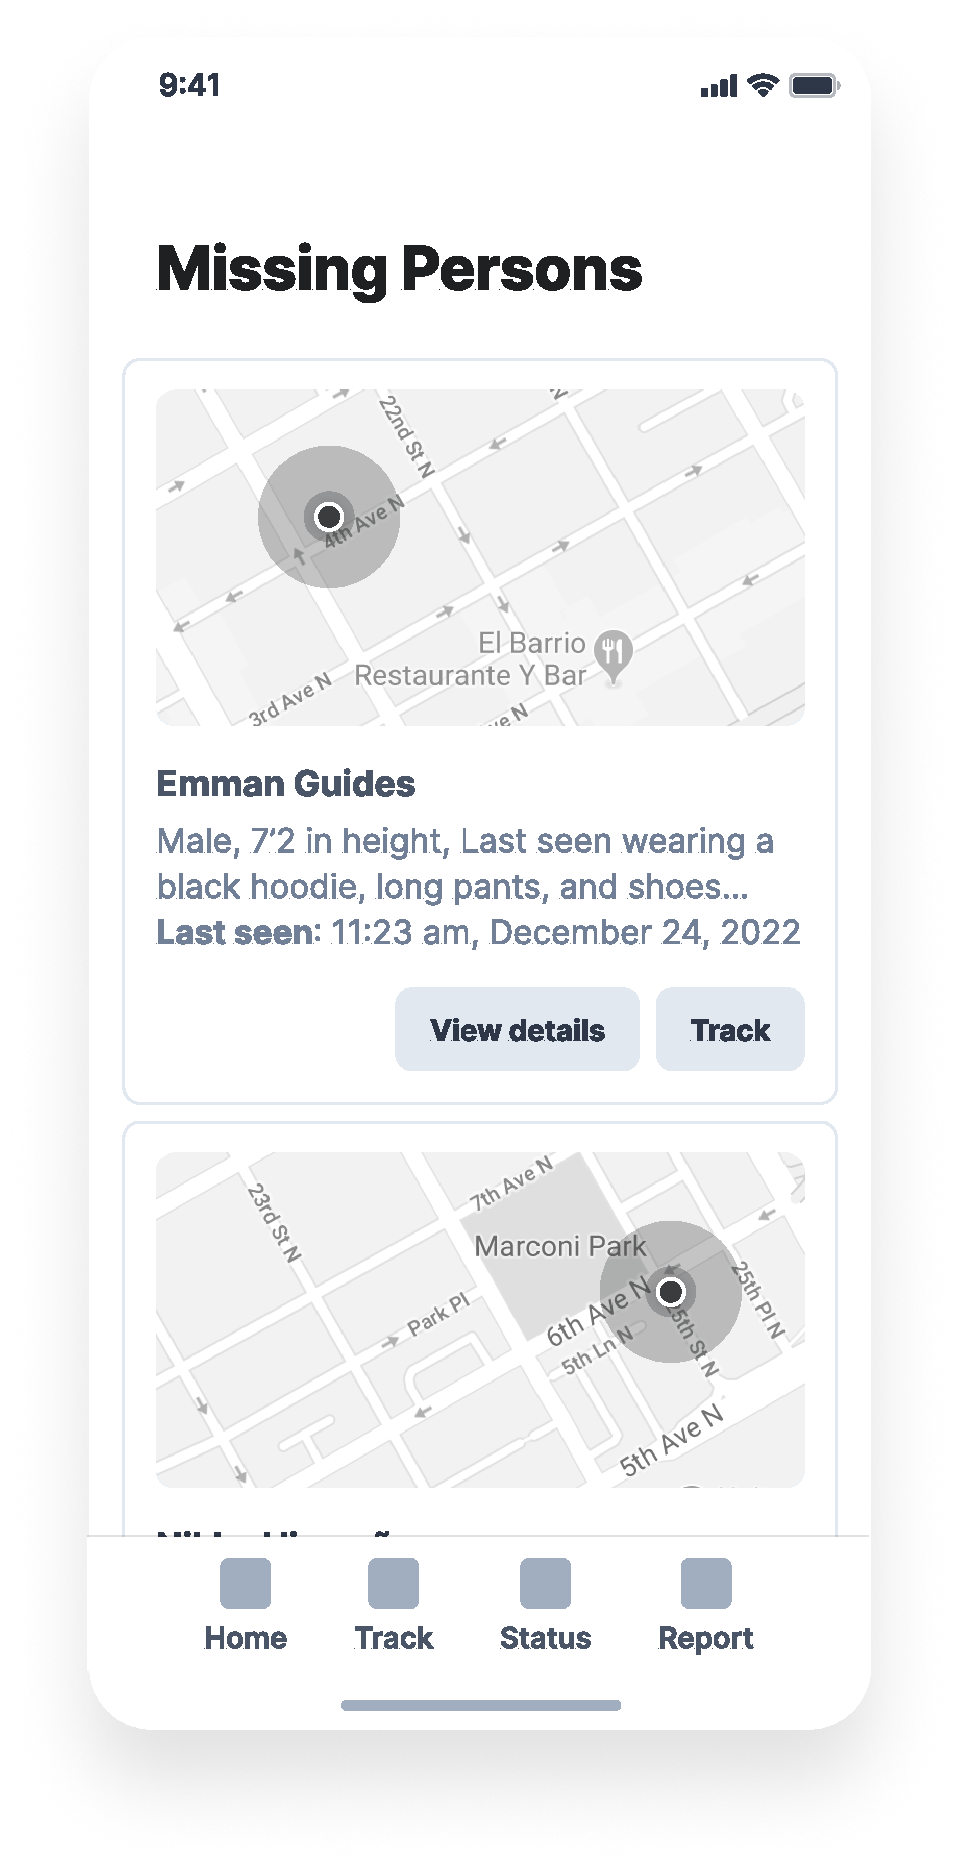
\includegraphics[scale=0.30]{interface/user/MissingPerson.pdf}
    \caption{Missing Persons Near Me}
    \label{fig:userMP}
\end{figure}
One of the features of the app is the consolidating all the missing reports in one view. Basically, this Figure \ref{fig:userMP} interface is a scrollable view for all Missing Persons Near Me feature which also redirects to Figure \ref{fig:userTracking} allowing maximization of the map for easy tracking. It would allow easy navigation of all missing reports and have a glimpse of any updates pertaining to the location that the MPs were seen. 

Obviously, the Report page is one of the integral parts of this application that would allow users to give necessary information in the event of a person missing. Figure 4.10 streamlines the reporting process done by the PNP and replicates their incident report so that verification is manageable. Input text fields will be used throughout this page. Accompanying it with dropdown menus for categorical information such as Gender, and Blood type. Physical indicators will have mostly text/paragraph input fields for elaborations and additional details that are needed to disclose such as body marks, tattoos, and the like.

\begin{figure}[!h]
    \centering
    \begin{minipage}[c]{0.50\linewidth}
        \centering
        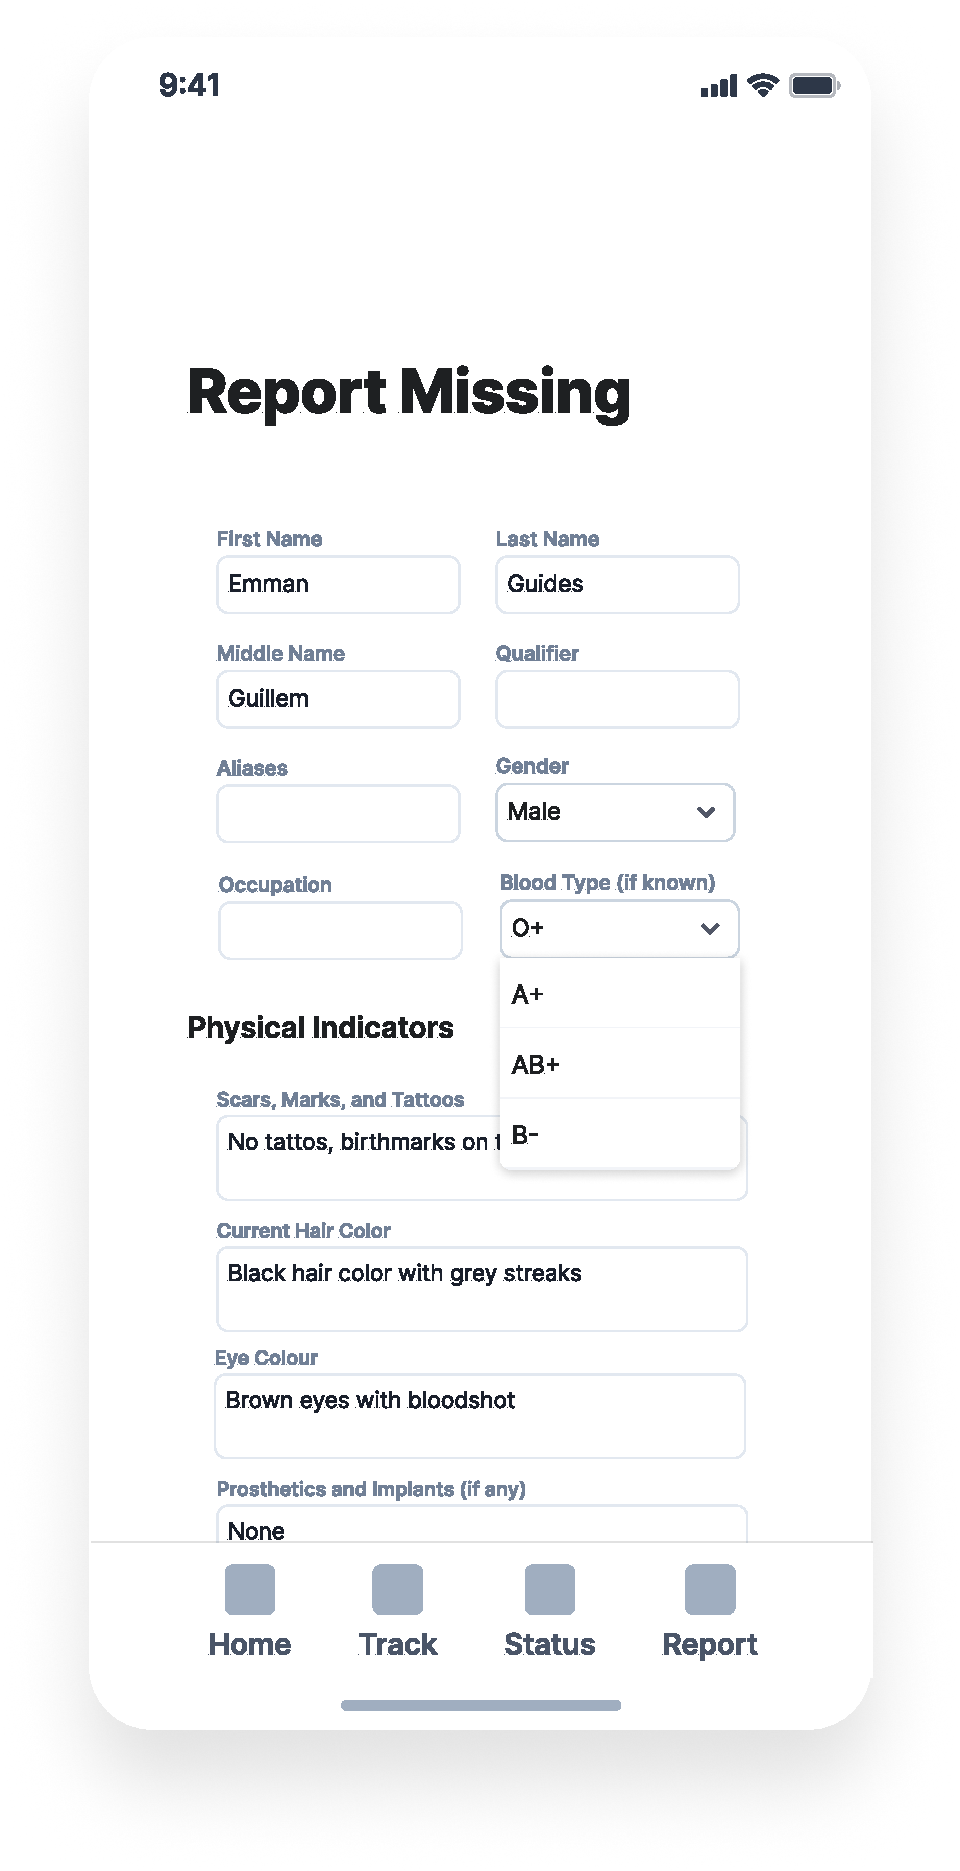
\includegraphics[scale=0.30]{interface/user/ReportMissing.pdf}
        \caption{Report Missing Section}
        \label{fig:userReportMP}
    \end{minipage}\hfill
    \centering
    \begin{minipage}[c]{0.50\linewidth}
        \centering
        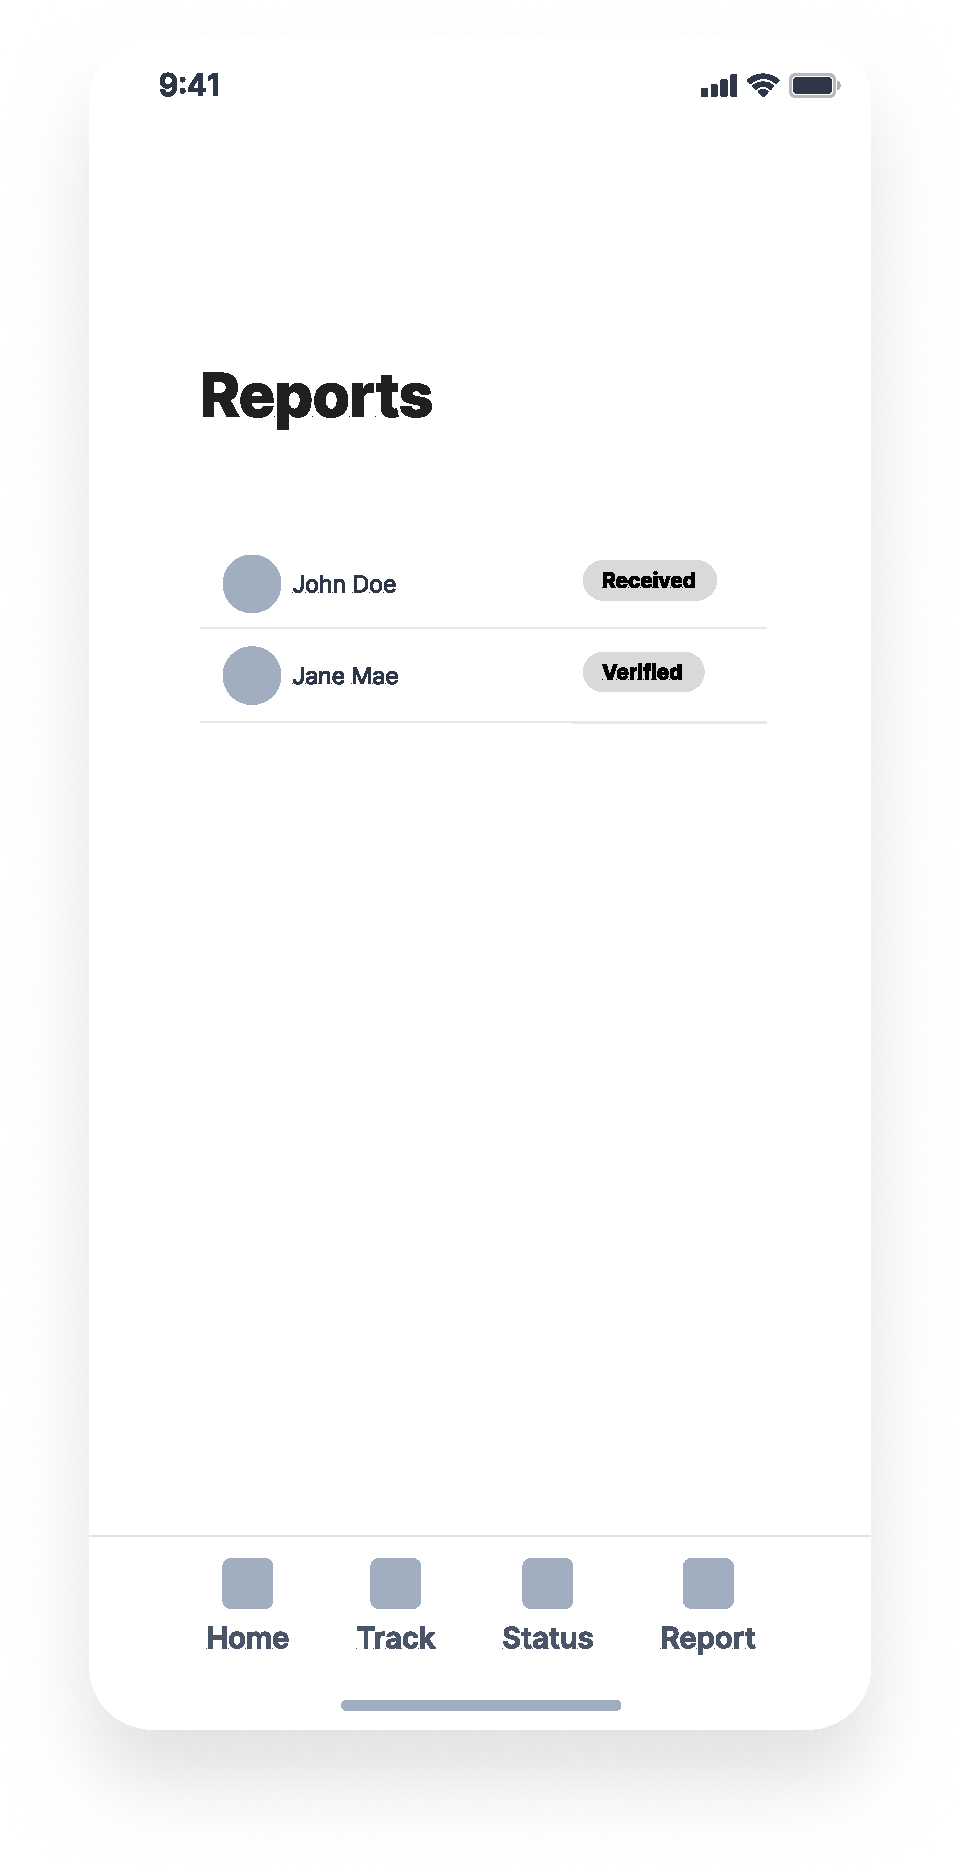
\includegraphics[scale=0.30]{interface/user/ReportStatus.pdf}
        \caption{Status Reports Section}
        \label{fig:userReportStatus}
    \end{minipage}
\end{figure}

\subsection{Companion-side}

\begin{figure}[t]
    \centering
    \begin{minipage}[c]{0.50\linewidth}
        \centering
    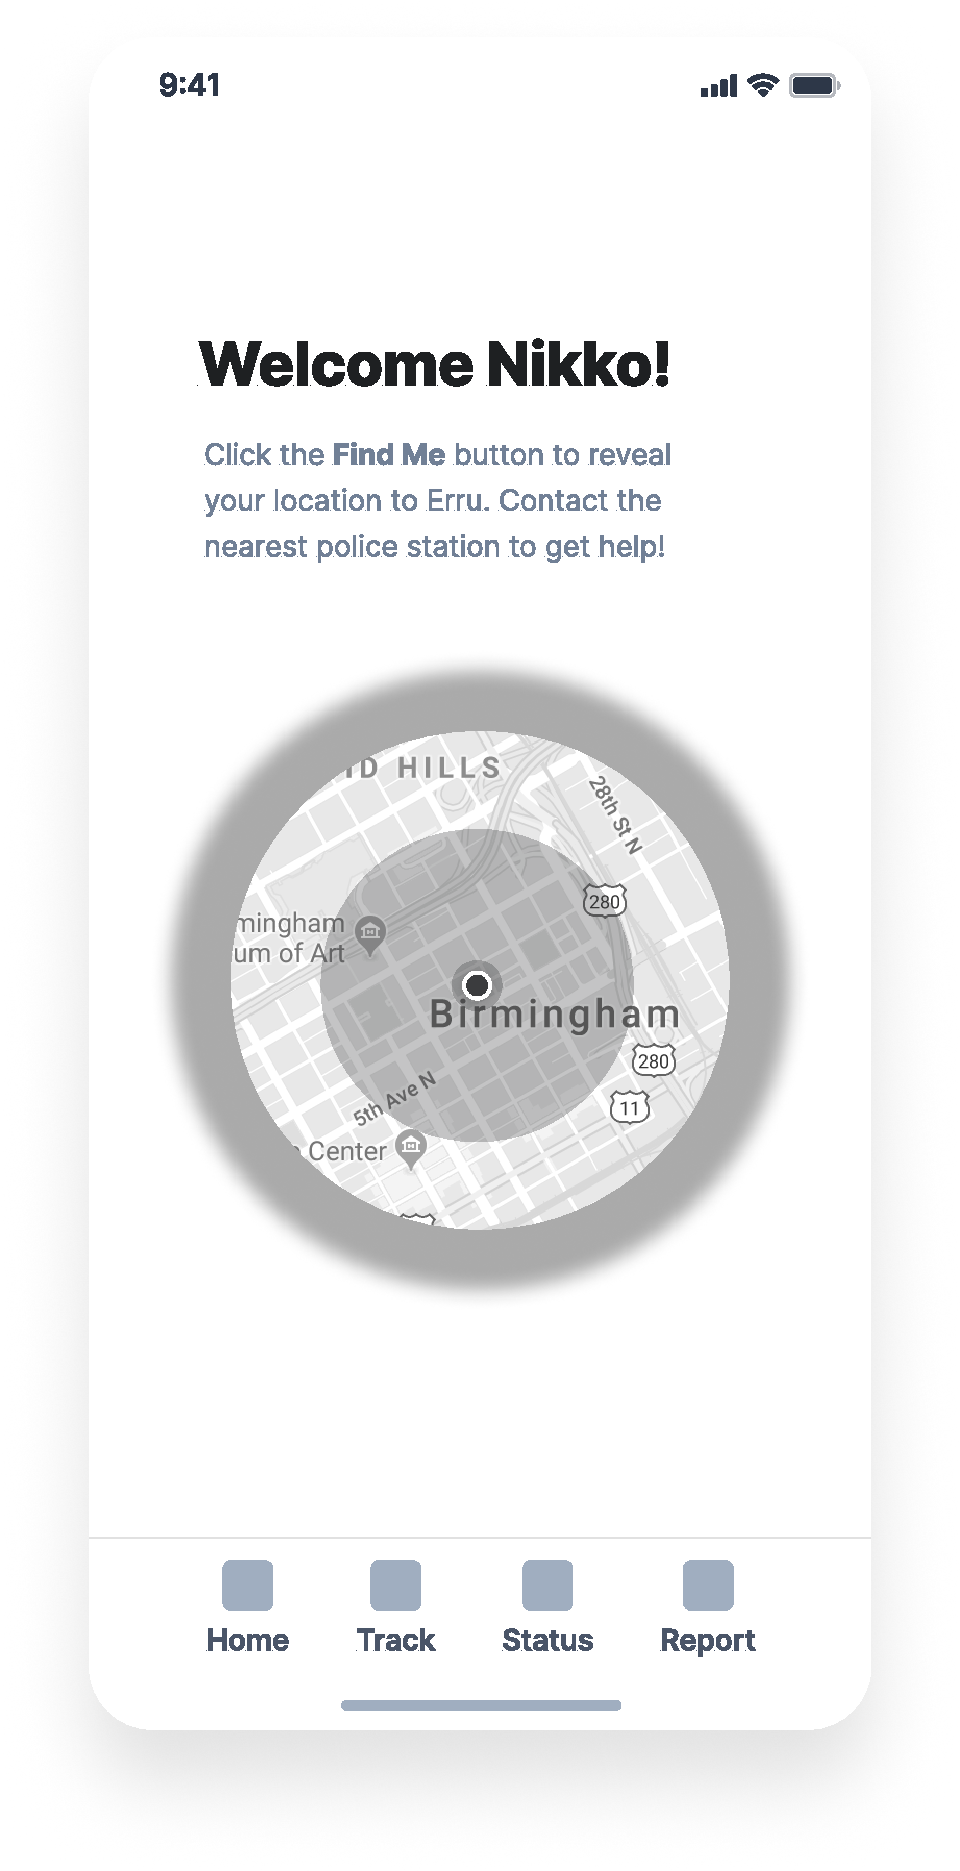
\includegraphics[scale=0.30]{interface/companion/FindMe.pdf}
    \caption{Find Me}
    \label{fig:companionFindMe}
    \end{minipage}\hfill
    \centering
    \begin{minipage}[c]{0.50\linewidth}
        \centering
        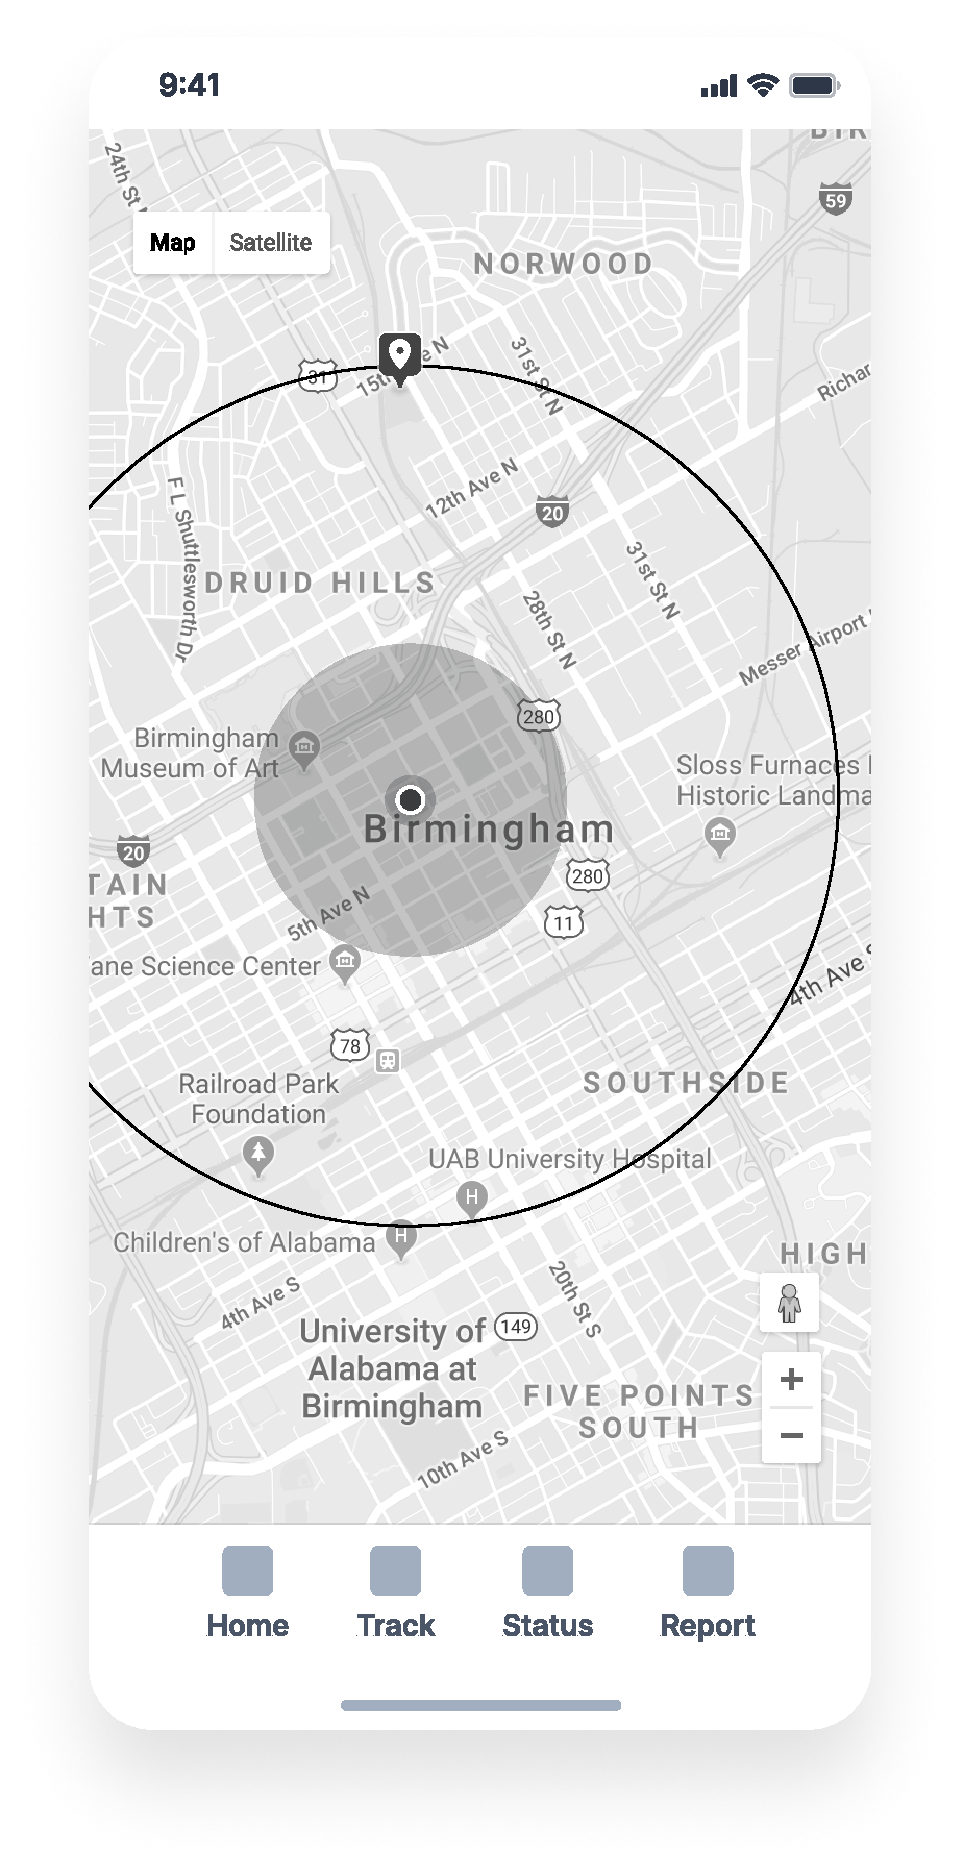
\includegraphics[scale=0.30]{interface/companion/ShowLocation.pdf}
        \caption{Show Location}
        \label{fig:companionShowLoc}
    \end{minipage}\hfill
    \centering
    \begin{minipage}[c]{0.50\linewidth}
        \centering
        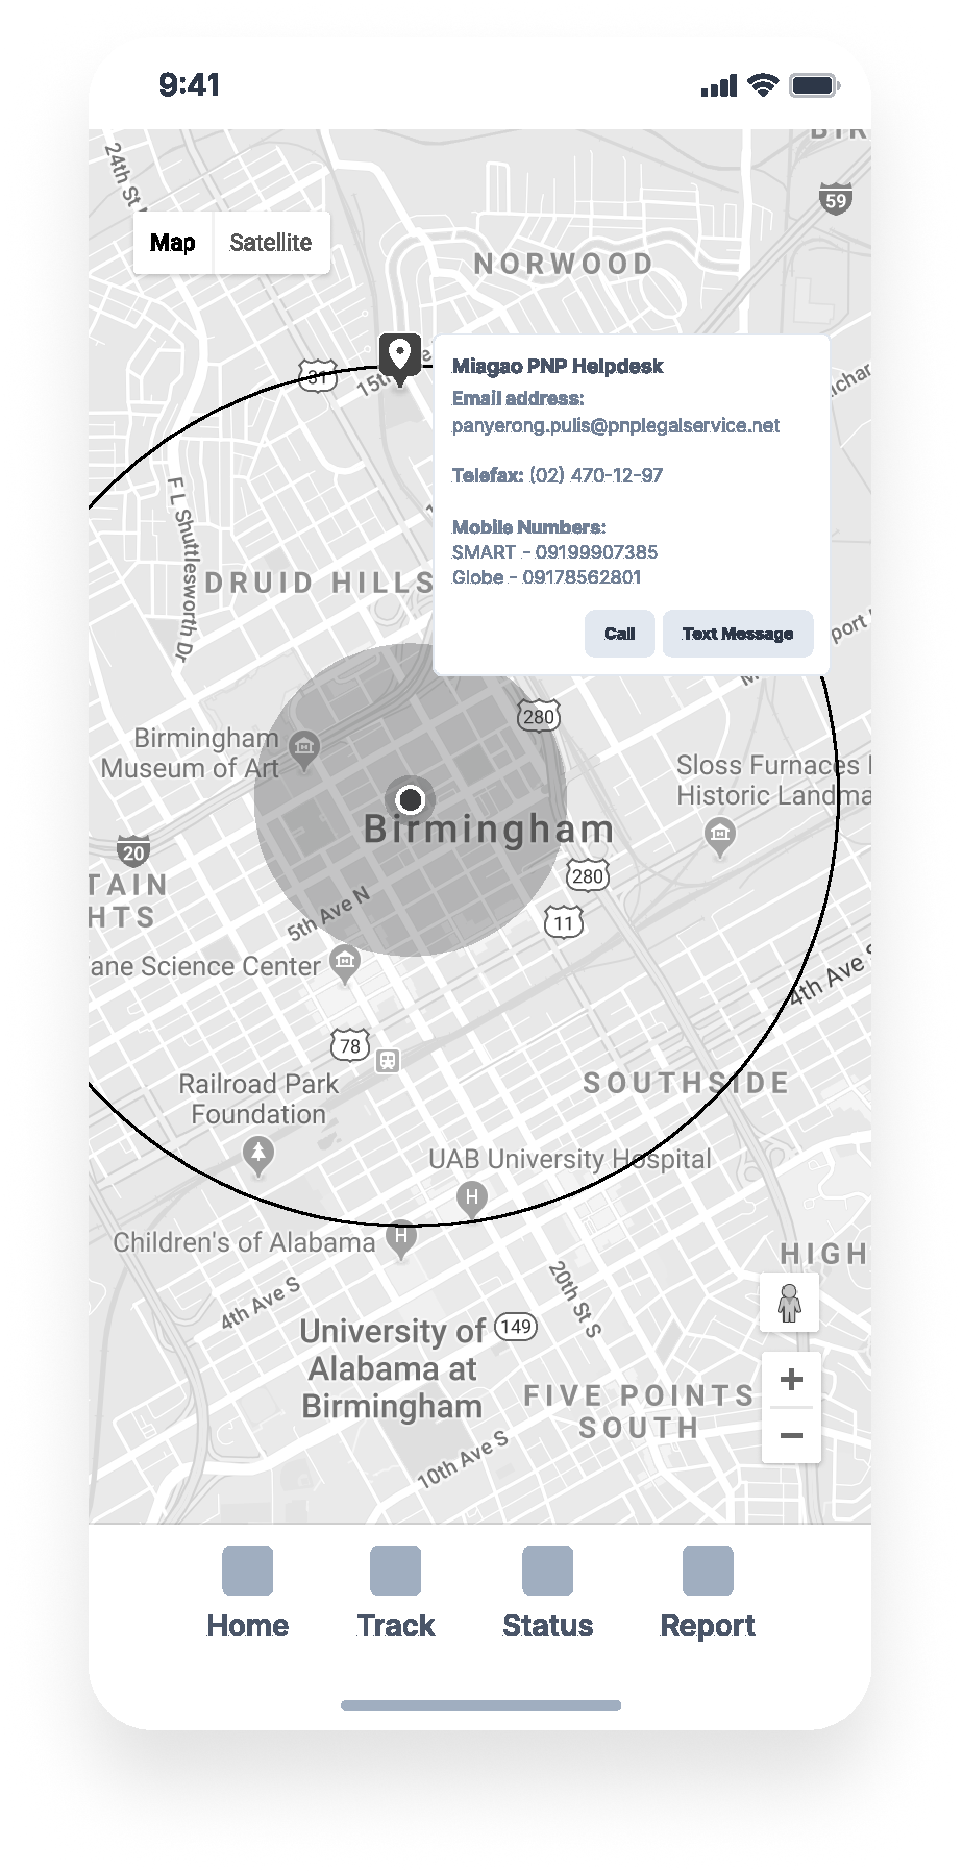
\includegraphics[scale=0.30]{interface/companion/GetHelp.pdf}
        \caption{Get Help}
        \label{fig:companionGetHelp}
    \end{minipage}
\end{figure}
Figure \ref{fig:companionFindMe} visualizes the interface for the “Find me” button. This will be the main feature of the companion-side app in which it will be centered at the home page after the login. In the event that the user is missing, the companion user can click the ”Find Me” button to let their paired User know their location, in case of an emergency. 

After the  “Find Me” button is activated, a map locating the user’s real-time location as shown in Figure \ref{fig:companionShowLoc} will be shown. Importantly, the companion can further leverage this by clicking nearby police stations within boundaries in order for them to be able to know the nearest Police Station they can possibly go to. Location markers will be visible in the map as long as it's the nearest police station from the user’s mark. Thus, companion users can easily contact the provided details of protective service and call or text message as shown in Figure \ref{fig:companionGetHelp} Get Help Section.